
\chapter{Título del tercer capítulo}
\label{chap:Infe}

\lipsum[10]


\section{Subsección 1}
\lipsum[100]. La Figura \ref{fig:subfiguras} presenta... La Figura \ref{fig:primera}... mientras que Figura \ref{fig:segunda}

\begin{figure}
	\centering
	\begin{subfigure}{0.45\textwidth}
		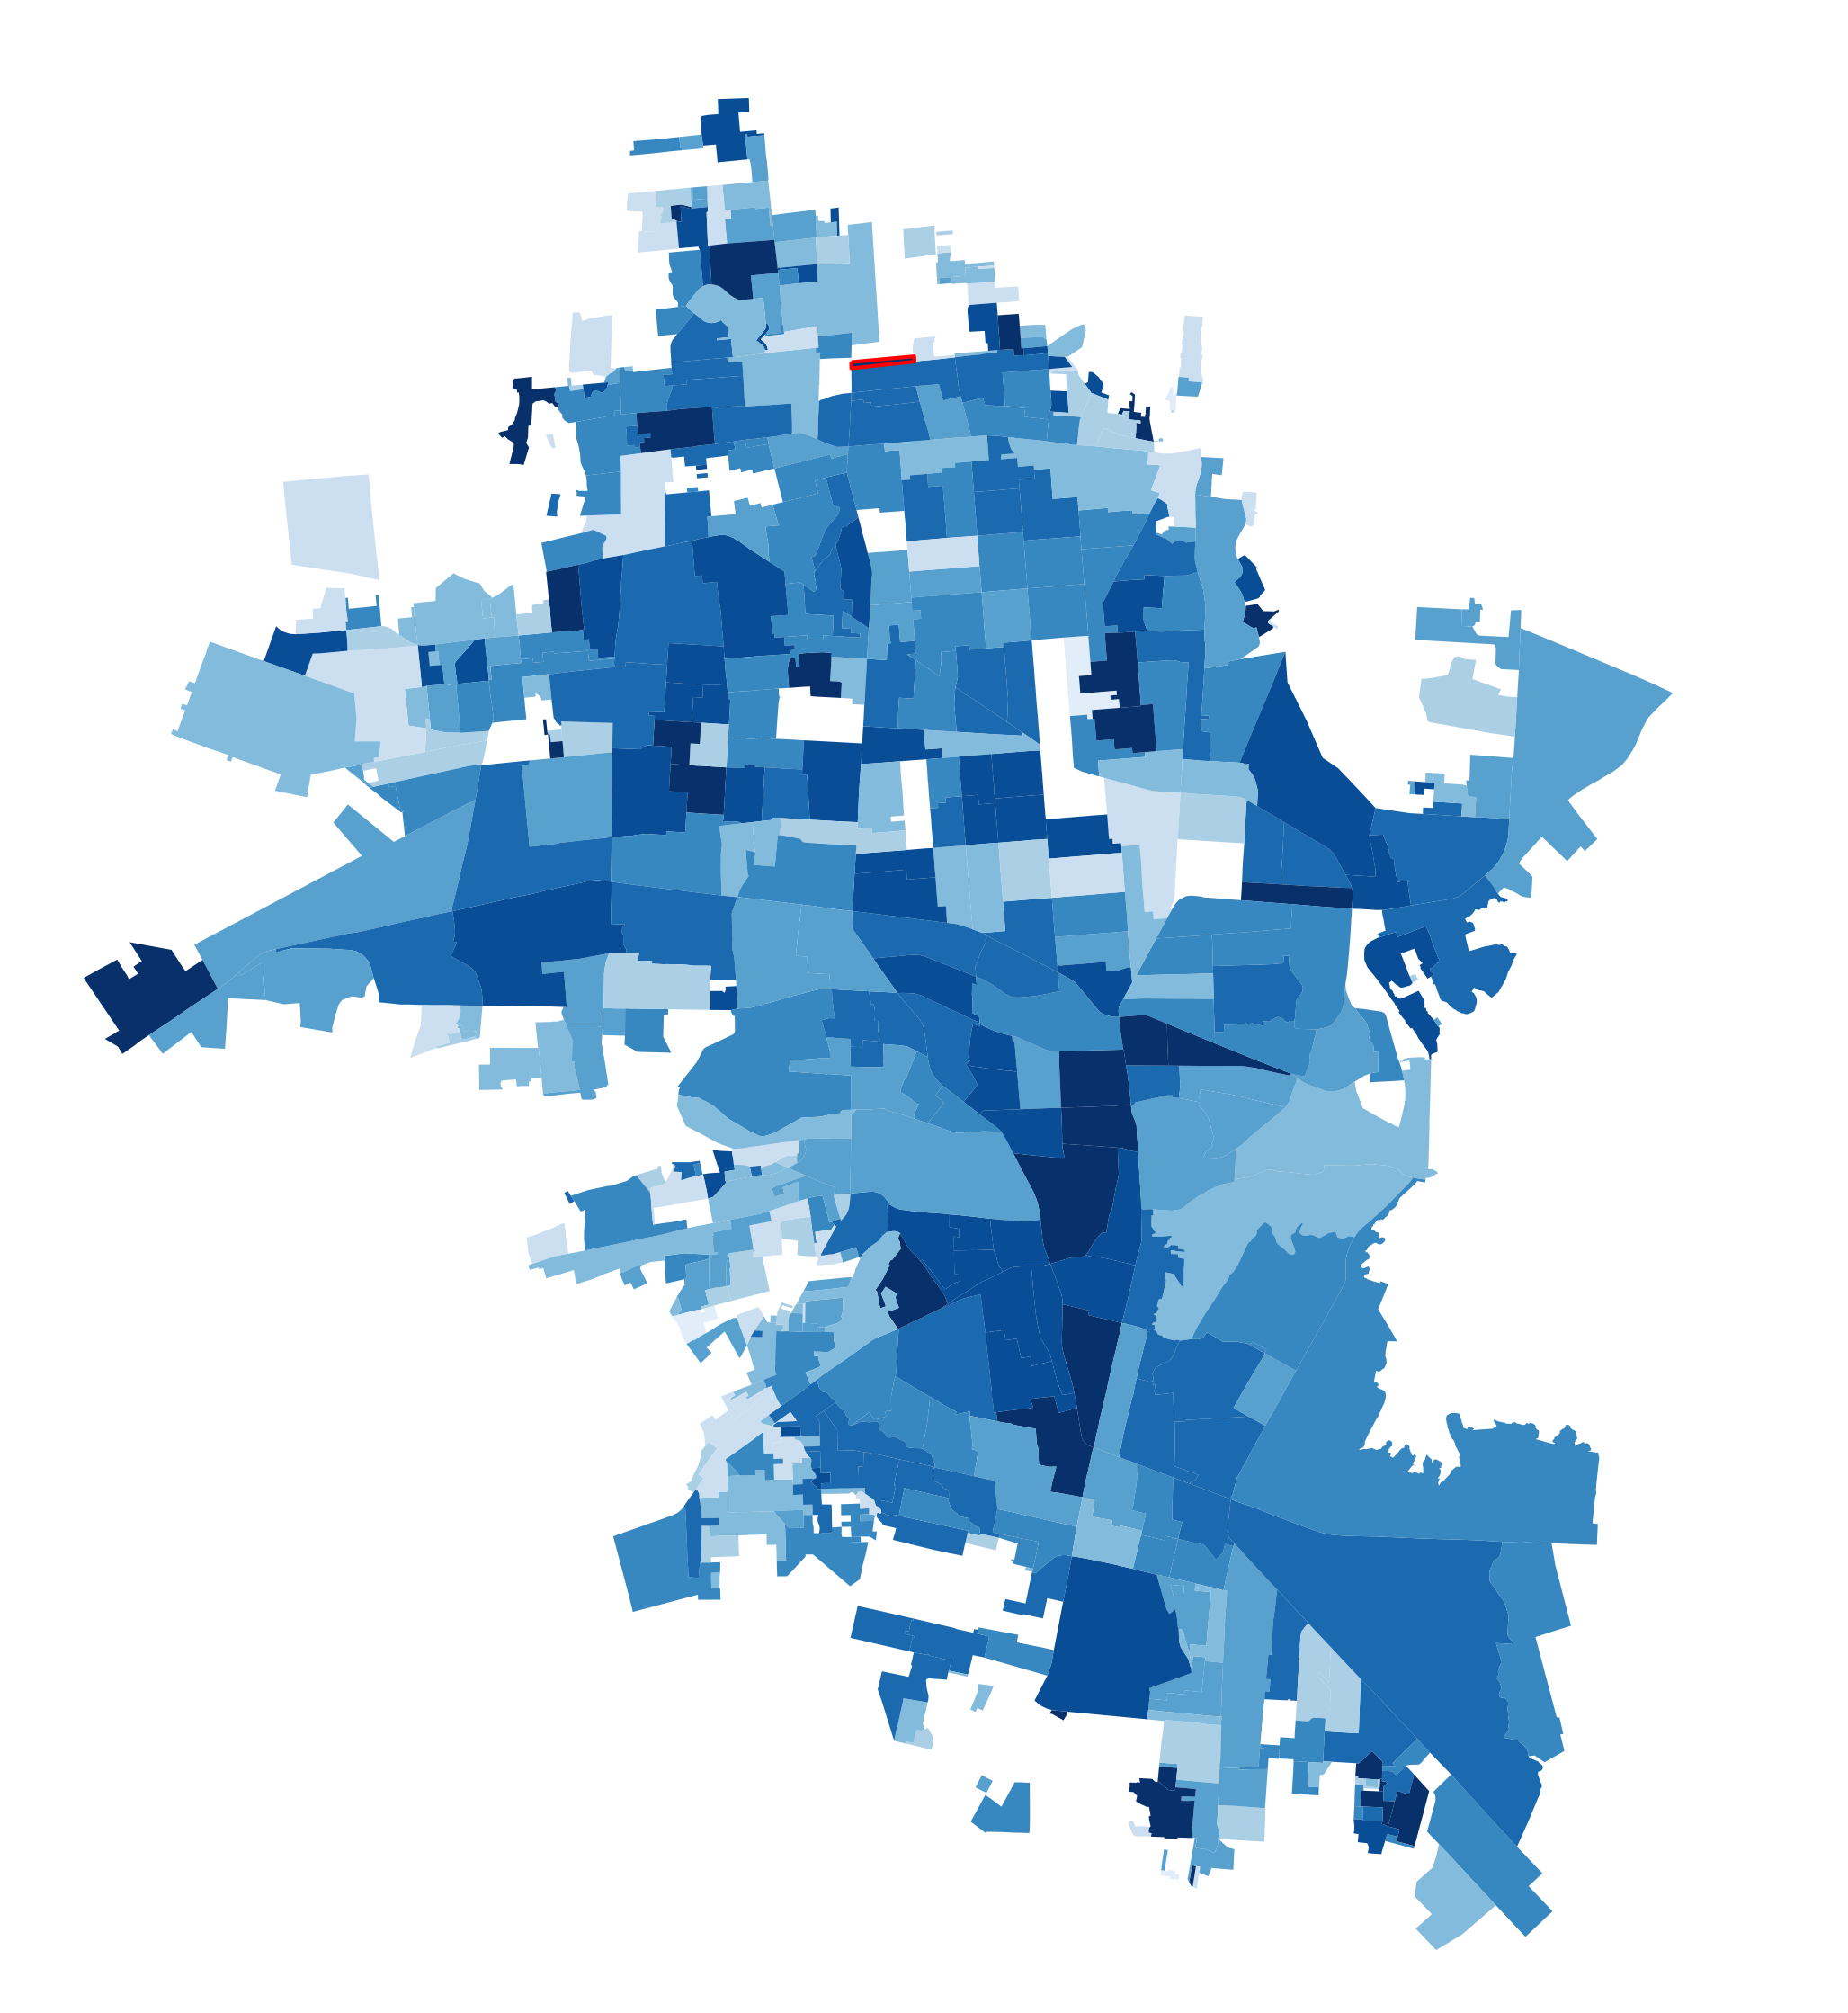
\includegraphics[width=\textwidth]{ejemplo-fig1.png}
		\caption{Descripción primera.}
		\label{fig:primera}
	\end{subfigure}
	\hfill
	\begin{subfigure}{0.45\textwidth}
		\center
		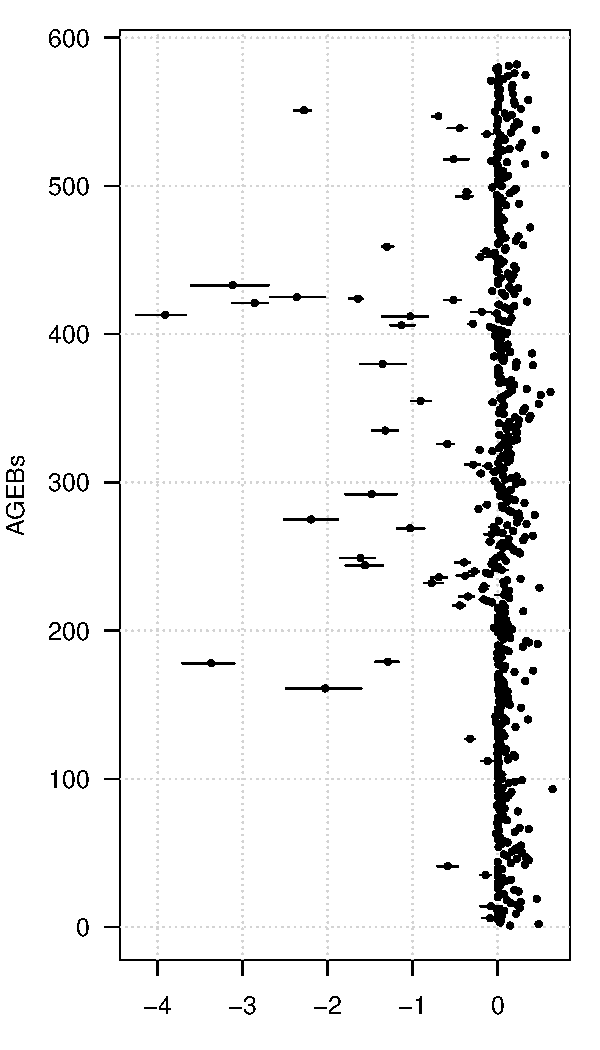
\includegraphics[width=0.7\textwidth]{ejemplo-fig3.pdf}
		\caption{Descripción segunda.}
		\label{fig:segunda}
	\end{subfigure}
	\hfill
	\caption{Ejemplo de dos figuras usando la función `subfigure' y el paquete `subcaption'.}
	\label{fig:subfiguras}
\end{figure}

\lipsum[1-4]






\subsection{Nombre de subsección 3-1-1}
\lipsum[100]
   \begin{table}
	\begin{center}
		\begin{tabular}{ c c  c   c c  c  c c c c c}
			%\hline 
			Evento & DIC & Eff & WAIC & logMLIK  & $\overline{CPO}$ & $\overline{PIT}$  \\ \hline \hline
			Semanas AR1 & 1938 & 117.3 & 1958 & -1052.5 &  0.020 &  0.500 \\
			D\'ias AR1 & 10567 & 188.7 & 10567 & -5389.3 &  0.068 & 0.524 \\
			Semanas RW & 1940 & 114.0 & 1964 &  -1047.4 &  0.014 & 0.369 \\
			D\'ias RW & 10575 & 175.5 & 10653 & -5382.7 & 0.068 & 0.524 \\
			\hline  
		\end{tabular}
	\end{center}
	\caption{Criterios para evaluación de modelos.}
	\label{tab:CriteriosTemporal}
\end{table}


\subsection{Nombre de subsección 3-1-2}
\lipsum[17]

\section{Subsección 2}
\lipsum[100] 




